\documentclass[conference,10pt]{IEEEtran}
\IEEEoverridecommandlockouts
\usepackage{graphicx,booktabs,amsmath,amssymb,multirow,xcolor,url,xspace}
\usepackage[hidelinks]{hyperref}
\hypersetup{pdftitle={로봇 양팔을 위한 에고센트릭 인간 시연, 제1부: 큐브 삼단 쌓기}, pdfauthor={Jeong Hwan Lee}}
\usepackage{tikz}
\usetikzlibrary{positioning,arrows.meta,fit,backgrounds}
\usepackage{fontspec}\setmainfont{Times New Roman}\usepackage{xeCJK}\setCJKmainfont[AutoFakeBold=2.5]{AppleMyungjo}\setCJKsansfont[AutoFakeBold=2.5]{Apple SD Gothic Neo}\setCJKmonofont{Apple SD Gothic Neo}\xeCJKsetup{CJKecglue={},CJKspace=true}
\newcommand{\mm}{\,mm\xspace}
\newcommand{\cmt}[1]{}

\begin{document}
\title{로봇 양팔을 위한 에고센트릭 인간 시연\\제1부: 큐브 삼단 쌓기}
\author{\IEEEauthorblockN{Jeong Hwan Lee}
\IEEEauthorblockA{기술 보고서, 버전 4, 2026년 10월 7일 \quad alnrg2arg@gmail.com\\
요약본. 제2부는 단일 팔 접근(approach) 데이터를 다룹니다. 코드, 결과, 샘플 데이터는 요청 시 제공합니다.}}
\maketitle

\begin{abstract}
본 연구는 손에 착용하는 UMI 방식 그리퍼로 기록한 에고센트릭(egocentric) 시연을 양팔 로봇 정책의 학습 데이터로 어디까지 바꿀 수
있는지 살펴본다. 균형을 맞춘 여섯 가지 순서로 큐브 세 개를 쌓는 시연 349개를 수집하고 두 세대에 걸쳐 처리하였다. 첫째, 에피소드별
IMU 스케일을 적용한 MASt3R-SLAM 손목 자세를 로봇 관절로 리타게팅하였다. 남은 세그먼트 561개로 학습한 0.9B X-VLA 모델은 held-out
인간 동작 중 움직이는 동작의 방향을 예측하지만(1.2\,s에서 코사인 0.90, 오차 39.9\mm), 정지 구간에서는 허위 동작을 예측하고 순서
지시문을 과제에 유용한 방식으로 사용하지 않는다. 둘째, 에피소드 전체를 실현 가능성 필터 없이 로봇 자신의 상대 데카르트(Cartesian)
액션 계약으로 변환하였다(에피소드 330개, 학습 행 48{,}411개). 계약을 공유하면 남은 인간--로봇 격차는 시각적이다. 에고 전용 모델은
로봇 프레임에서 유용한 액션 방향을 주지 못하며, 입력을 맞바꾸어 보면 격차는 손목 이미지에 있다. 초기값으로서 에고 사전학습은 로봇
에피소드 312개와 30개 모두에서 초기 로봇 파인튜닝을 빠르게 하지만, 학습 손실상의 이점은 사라진다(312개에서는 60k 스텝까지, 30개에서는
약 100k--200k 스텝에서). 로봇 에피소드 312개로 파인튜닝한 에고 초기화 모델은 폐루프에서 큐브 세 개를 쌓았으나, 시도 횟수를 세지
않았으므로 성공률이 아닌 시연으로 보고한다.
\end{abstract}

\section{서론}
에고센트릭 인간 시연은 로봇 원격조작보다 수집 비용이 낮고, UMI~\cite{chi2024umi}와 같은 손 착용 그리퍼는 인간의 엔드이펙터를 로봇과
비슷하게 만든다. 이러한 데이터가 특정 로봇으로 전이되는지는 캘리브레이션, 메트릭 자세 복원, 로봇 액션 공간으로의 변환, 필터링에 달려
있으며, 각 단계는 정책이 학습하는 내용을 드러나지 않게 바꿀 수 있다. EgoMimic~\cite{kareer2024egomimic}과
MimicPlay~\cite{wang2023mimicplay}는 인간 영상으로부터의 폐루프 성능 향상을 보고하는 반면, 본 연구는 실제 데이터로 이 사슬을 한 번
완주한 과정을 점검한다. 질문은 좁다. \emph{모든 처리를 거친 뒤, 사전학습된 vision-language-action(VLA) 모델은 에고센트릭 인간
시연으로부터 로봇이 실행 가능한 액션 구조를 얼마나 학습하며, 그것이 로봇 파인튜닝에 도움이 되는가?} 평가는 대부분 오프라인이거나 학습
손실 기반이다. 배치가 기록되지 않았고 여섯 순서 모두 학습에 등장하므로 공간 일반화도 과제 순서 일반화도 검증하지 않는다. 이 요약본은
전체 보고서(저장소에 보관)를 압축하고 실행 상태를 2026년 10월 7일 기준으로 갱신한다.

\section{데이터와 자세}\label{sec:data}
\textbf{장치와 과제.} 양손에 각각 HandUMI 장치를 착용한다. 1080p30 어안(fisheye) 손목 카메라, 200\,Hz IMU, 조(jaw) 인코더로
구성되며, 고정된 Logitech C922가 탁자를 기록한다. 50\mm{} 큐브 세 개를 지시문이 지정하는 여섯 순서 중 하나로 접시 위에 쌓는다.
조작자 한 명이 2026년 9월 15--17일에 15개 세션에서 에피소드 349개(2.20\,h, 중앙값 23.05\,s)를 기록하였다. 다음 순서는 가장 적게
수집된 순서로 정해지므로(순서당 51--64개) 순서는 무작위가 아니라 균형을 맞춘 것이다. 큐브 배치는 수동 리셋을 통해 달라졌지만 기록되지
않았다(그림~\ref{fig:dataset}). 이후 로봇 유사 세션(HRL80)에서 에피소드 60개(순서당 10개)를 추가하였다.

\begin{figure*}[t]
\centering
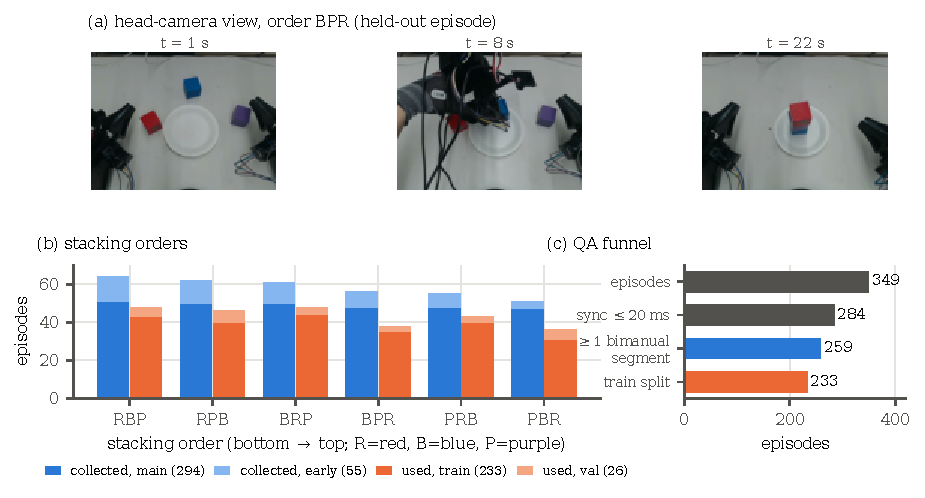
\includegraphics[width=\textwidth]{figures/fig2_dataset.pdf}
\caption{데이터셋 설계. (a) held-out 에피소드(순서 BPR)의 1, 8, 22\,s 시점 헤드 카메라 프레임. (b) 쌓기 순서별 에피소드 수: 수집 시와
1세대 처리 후. (c) 에피소드 수준 퍼널.}
\label{fig:dataset}
\end{figure*}

\textbf{캘리브레이션.} Kannala--Brandt 어안 내부 파라미터, Kalibr~\cite{furgale2013kalibr} 카메라--IMU 캘리브레이션(시간 오프셋
30.2, 32.8\,ms, 평균 재투영 오차 6.0, 5.6\,px로 높은 편이어서 자세 정확도를 별도로 검증한다), 장치 하나에서 캘리퍼로 측정한
카메라--TCP 변환을 사용한다.

\textbf{손목 자세.} UMI의 장면별 ORB-SLAM3 지도는 본 데이터에서 실패하였다(커버리지 중앙값 0.03, 잦은 위치 역전). RGB 영상만으로
MASt3R-SLAM~\cite{murai2025mast3rslam}을 실행하고 에피소드마다 IMU로부터 메트릭 스케일을 복원한다. ArUco 벤치마크 에피소드 14개에서
커버리지는 1.00(대 0.03), 스케일 오차 p50/p90은 4.6/17.0\%(단일 전역 상수는 18.5/23.8\%), 회전 오차 p50은 0.84\textdegree{}, 16스텝
상대 위치 오차 p90은 11.3\mm{}이다.

\section{1세대: 관절 공간 리타게팅}\label{sec:gen1}
\textbf{처리.} 각 TCP 궤적을 IK로 reBot B601 6-DoF 팔에 리타게팅하고, 고정된 로봇 시작 자세에 다시 앵커링한다. 65개 에피소드가
$\le$20\,ms 동기화 요건을 통과하지 못한다. 양팔 65프레임 후보 세그먼트 1{,}306개 중 677개는 로봇 작업공간을 벗어나고, 50개는 메트릭
검사에, 18개는 IK에 실패하여 에피소드 259개에서 561개(43.0\%)가 남으며, 이를 에피소드 단위로 학습 233 / 검증 26으로 분할한다.
X-VLA~\cite{zheng2025xvla}(파라미터 879M, \texttt{xvla-base}에서 시작, LeRobot~\cite{cadene2024lerobot} 사용)를 300k 스텝 파인튜닝하여,
세 시점, 지시문, 14-D 상태로부터 관절 변위 30스텝 청크를 예측하게 한다.

\begin{table}[t]
\centering\footnotesize\setlength{\tabcolsep}{5pt}
\caption{오프라인 held-out 결과, 최종 300k 체크포인트(에피소드 26개). TCP 오차: FK 위치 오차 중앙값(mm). MAE: 관절 MAE(deg),
괄호 안은 무동작 예측기.}
\label{tab:results}
\begin{tabular}{@{}llccc@{}}
\toprule
부분집합 & 지표 & $k{=}1$ & $k{=}8$ & $k{=}30$ \\
\midrule
전체 (798) & TCP 오차 & 1.5 & 2.2 & 5.7 \\
 & MAE & 0.30 (0.15) & 0.42 (0.25) & 0.97 (0.51) \\
\midrule
동작 (187) & TCP 오차 & 11.2 & 19.4 & 39.9 \\
 & MAE & 2.02 (2.32) & 3.29 (4.38) & 6.59 (8.68) \\
 & cosine & 0.72 & 0.84 & 0.90 \\
\bottomrule
\end{tabular}
\end{table}

\textbf{오프라인 결과}(표~\ref{tab:results}, 그림~\ref{fig:eval}). 샘플의 77\%가 거의 정지 상태이므로 전체 샘플의 오차는
작다(1.5--5.7\mm). 20\mm 이상 움직이는 23.4\%의 샘플에서는 $k{=}30$(1.2\,s)의 오차가 39.9\mm, 방향 코사인이 0.72에서 0.90으로
오르며, 관절 MAE는 무동작 예측기보다 13--32\% 낮다($k{=}30$에서 6.59 대 8.68\textdegree). 전체 샘플에서는 정책이 무동작 예측보다
\emph{나쁘다}. 정지 구간에서 미세하게 움직인다(creep). \textbf{Prompt swap.} 여섯 순서 지시문은 $k{=}30$ 예측을 4.8\mm{}만큼
움직이는데(노이즈 퍼짐의 50$\times${}이지만 예측 변위 62\mm{}의 8\%), 올바른 지시문의 평균 순위는 6개 중 3.55(우연 수준 3.5)이다.
모델은 순서를 과제에 유용한 방식으로 사용하지 않는다.

\begin{figure*}[t]
\centering
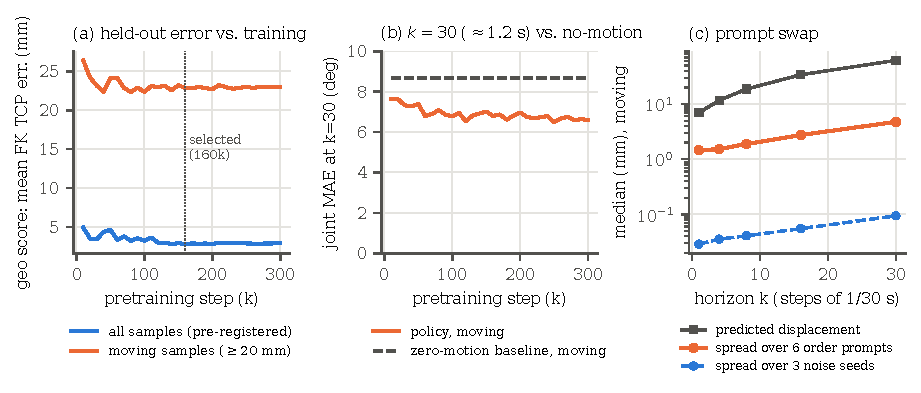
\includegraphics[width=0.92\textwidth]{figures/fig4_eval.pdf}
\caption{1세대 오프라인 평가. (a) 학습 과정에 따른 전체 대 동작 샘플의 geo score. (b) 동작 샘플의 $k{=}30$ 관절 MAE, 정책 대
무동작 예측기. (c) Prompt swap: 여섯 지시문 간 퍼짐 대 세 노이즈 시드 간 퍼짐.}
\label{fig:eval}
\end{figure*}

\textbf{리타게팅 v2와 파인튜닝.} 단일 시작 앵커가 주된 손실 원인이었다. 가장 가까운 실현 가능한 로봇 궤적 윈도를 검색하면(로봇
에피소드 30개로 보정하고 다른 120개에서 측정) 사용 가능한 세그먼트가 36.5\%에서 56.1\%로 오르고(표~\ref{tab:retarget}), 자세가 실제
로봇 자세에 가까워진다(최근접 이웃 거리 1.49$\to$0.27\,rad, 시작 클러스터 1$\to$100). 로봇 유사 재수집은 실시간 손목 회전 속도를
절반으로 줄였으나 사용 가능한 세그먼트는 58.9\%로 오르는 데 그쳤다. 한계는 수집 방식이 아니라 작업공간 배치이다. 로봇 에피소드
150개로 파인튜닝했을 때 에고 초기화 모델의 geo score는 base 모델에서 학습한 모델보다 10\% 낮지만(95\% CI 5.6--14.7\%), 두 학습 세트
모두에 포함된 에피소드에서만 측정한 것이므로 이는 일반화가 아니라 피팅을 측정한다.

\begin{table}[t]
\centering\footnotesize\setlength{\tabcolsep}{3.5pt}
\caption{후보 세그먼트 1{,}229개에 대한 리타게팅 변형 비교, held-out 로봇 에피소드 120개 기준. NN: 로봇 자세까지의 최근접 이웃 관절
거리(rad, p50/p90).}
\label{tab:retarget}
\begin{tabular}{@{}lccc@{}}
\toprule
변형 & 사용 가능 & NN p50 / p90 & 시작 클러스터 \\
\midrule
v1 단일 앵커 & 36.5\% & 1.49 / 1.55 & 1 \\
v2-K 다중 시드 IK & 66.6\% & 1.21 / 1.60 & -- \\
v2-Kr + 자세 페널티 & 67.0\% & 0.44 / 0.74 & -- \\
v2-TR 윈도 검색 & 56.1\% & 0.27 / 0.45 & 100 \\
\bottomrule
\end{tabular}
\end{table}

\section{2세대: 데카르트 에고 데이터}\label{sec:gen2}
\textbf{계약.} 관절 리타게팅은 동작의 3분의 1에서 절반을 제거했고, 로봇 정책과 다른 액션 공간을 썼다. 2세대는 각 손목 궤적을 로봇
데이터의 표현으로 직접 변환한다. 행은 15\,Hz이며, 액션 청크는 상대 자세 16개 $T(t)^{-1}T(t+k\Delta)$, $\Delta=50.05$\,ms(0.8\,s)로
원시 30\,Hz 궤적에서 보간한다. 팔마다 위치, 6-D 회전, 그리퍼(20차원, ``CART20'')이고 32-D 헤드의 나머지는 0으로 두며, 상태는 각 팔의
과제 시작에 대한 상대값이다. 원천은 원래 에피소드 273개와 HRL80 에피소드 60개이며, IMU 스케일 검사 후 330개가 남고, 작업공간이나 IK
필터는 없다.

\textbf{드러나지 않는 자세 점프.} 에고 상태에는 로봇 데이터에 없는 100\mm 초과의 점프가 있었다. 30\mm{}를 넘는 겉보기 점프
2{,}598개 중 1{,}482개는 인접하지 않은 행 사이의 시간 공백이었다. 나머지는 추적 손실 플래그 없이 일어난 실제 MASt3R-SLAM 한 프레임
점프로, 시작에 앵커링된 이후 모든 상태를 손상시킨다. 이런 점프 이후를 잘라내면 학습 에피소드 297개, 행 48{,}411개($-6.20$\%)가
남고, 인접 행 사이의 최대 스텝은 422.5에서 90.5\mm{}로 줄어든다.

\textbf{에고 대 로봇.} 로봇 IK는 에고 위치의 99.7\%(왼쪽)와 99.5\%(오른쪽)에 도달한다. 에고 손은 더 작은 작업공간을 쓰고, 두 손이
동시에 정지해 있는 경우가 훨씬 잦다(샘플의 19.5\% 대 2.4\%). 가장 큰 차이는 시각적이다. 손목 이미지 선명도(Laplacian 분산)
중앙값이 에고 어안 시점에서는 1{,}854/1{,}487, 로봇 손목 카메라에서는 59/64이다.

\section{로봇으로의 전이}\label{sec:transfer}
모든 실행은 하나의 레시피를 쓴다. X-VLA, 액션 차원 0--19에만 손실, 배치 8, 8-bit AdamW(정책 학습률 $10^{-4}$), bf16, seed 1000이며,
파인튜닝은 로봇 정규화 통계를 쓴다. R312c는 같은 과제의 로봇 원격조작 에피소드 312개이다.

\textbf{어떤 soft prompt인가?} X-VLA는 embodiment id로 soft prompt를 선택한다. 공개 base 가중치에서는 슬롯 10--17만 학습된 적이
있으며, 본 연구에서 쓴 id 0과 6은 학습되지 않은 슬롯이었다. 아래 모든 실행은 사용되지 않은 슬롯 20을 쓴다.

\begin{table}[t]
\centering\footnotesize\setlength{\tabcolsep}{3.2pt}
\caption{에고 전용 체크포인트(40k)에서 이미지와 상태가 서로 다른 도메인에서 올 때의 $k{=}4/8/16$ 방향 코사인 중앙값(왼쪽 $|$
오른쪽).}
\label{tab:ablation}
\begin{tabular}{@{}lcc@{}}
\toprule
이미지 + 상태 & 왼쪽 $k$=4/8/16 & 오른쪽 $k$=4/8/16 \\
\midrule
에고 + 에고 & 0.87 / 0.91 / 0.92 & 0.89 / 0.94 / 0.84 \\
에고 + 로봇 & 0.76 / 0.81 / 0.90 & 0.72 / 0.69 / 0.72 \\
로봇 + 로봇 & 0.36 / 0.30 / $-$0.01 & 0.19 / 0.02 / $-$0.15 \\
로봇 + 에고 & 0.16 / 0.24 / $-$0.16 & 0.49 / 0.33 / $-$0.03 \\
\bottomrule
\end{tabular}
\end{table}

\textbf{격차는 손목 이미지에 있다.} 로봇 프레임 120개에서 에고 전용 모델(40k 스텝)의 0.4\,s 방향 코사인 중앙값은
$-0.05$/$-0.03$(왼쪽/오른쪽)으로, 로봇으로 학습한 기준 모델의 $+0.81$/$+0.77$에 못 미치며, 어떤 축 또는 팔 교환도 이를 $+0.16$ 위로
올리지 못한다. 도메인 간에 입력을 맞바꾸면(표~\ref{tab:ablation}), 에고 모델은 에고 이미지를 받으면 어떤 상태가 주어지든(로봇 상태
포함) 0.69--0.90의 코사인을 유지하고, 로봇 이미지를 받으면 상태와 관계없이 $-0.25$에서 $+0.49$ 사이로 떨어진다. 에고 손목 프레임을
로봇 유사 핀홀 시점으로 다시 렌더링하면(ROBOT100) 선명도가 181/132로 낮아지지만 여전히 로봇의 2--3$\times${}이다. 이 데이터로
300k 사전학습을 수행하여 10월 5일에 끝났다(학습 손실 0.007).

\textbf{로봇 에피소드 312개에서의 초기화.} 동일한 데이터, 스케줄, 시드로 base 모델(A)과 50k 에고 체크포인트(B)에서 R312c로
파인튜닝하면, B는 3.9$\times${} 낮은 손실에서 출발한다(스텝 200에서 A 0.945, B 0.244). 비율 B/A는 처음 5k 스텝에서 0.49,
5k--20k에서 0.875, 20k--40k에서 0.95이며, 60k에서 두 값이 동률이다(0.0733 대 0.0745, 그림~\ref{fig:egoinit}). 학습 손실만이며
조건당 시드 하나이고, A와 B의 held-out 또는 폐루프 비교는 없다.

\begin{figure*}[t]
\centering
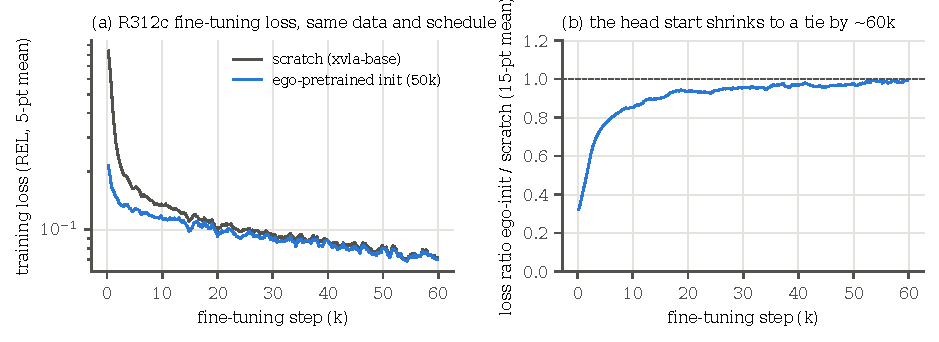
\includegraphics[width=0.72\textwidth]{figures/fig5_ego_init_loss.pdf}
\caption{같은 데이터·스케줄·시드에서 base 모델과 50k 에고 체크포인트로부터의 R312c 파인튜닝 비교. (a) 학습 손실. (b) 비율. 1
미만이면 에고 초기화에 유리하다.}
\label{fig:egoinit}
\end{figure*}

\textbf{로봇 에피소드 30개에서의 초기화.} 인간 데이터가 중요해야 할 영역을 검증하기 위해, R30(R312c 에피소드 150--179, 프레임
17{,}600개, 600k 스텝 스케줄)으로 base 모델과 ROBOT100 사전학습의 100k 및 300k 스텝에서 파인튜닝하였다(표~\ref{tab:r30},
그림~\ref{fig:r30}). 두 에고 초기화 모두 scratch 손실의 절반 미만에서 출발한다(1k--5k 윈도 비율 0.544와 0.493). 100k 초기화는 약
100k 스텝까지 동등해지고(50k--100k에서 0.970, 100k--150k에서 1.021), 300k 초기화는 약 200k에서 동등해진다. 100k 체크포인트는
스케줄의 중간이고 300k 조건은 다른 GPU와 PyTorch 버전에서 실행되었으므로 조건들은 정확한 쌍둥이 실행이 아니다. 세 실행은
139--214 epoch 후 471k, 305k, 310k 스텝에서 중단하였다. 모든 조건이 30개 에피소드를 암기한다. R30 체크포인트는 아직 로봇에서
실행되지 않았다.

\begin{table}[t]
\centering\footnotesize\setlength{\tabcolsep}{4pt}
\caption{R30 파인튜닝: 맞춘 스텝에서의 학습 손실과 scratch 대비 윈도 평균 비율($<$1이면 에고에 유리). 조건당 시드 하나.}
\label{tab:r30}
\begin{tabular}{@{}lccc@{}}
\toprule
스텝 / 윈도 & Scratch & Ego-PT 100k 초기화 & Ego-PT 300k 초기화 \\
\midrule
200 & 0.801 & 0.239 & 0.446 \\
10k & 0.065 & 0.056 & 0.040 \\
100k & 0.009 & 0.009 & 0.007 \\
\midrule
비율 1k--5k & & 0.544 & 0.493 \\
비율 50k--100k & & 0.970 & 0.856 \\
비율 100k--150k & & 1.021 & 0.914 \\
\bottomrule
\end{tabular}
\end{table}

\begin{figure*}[t]
\centering
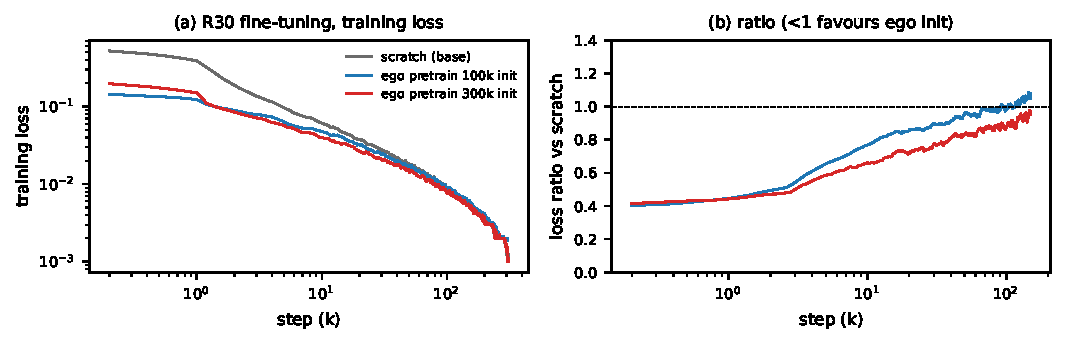
\includegraphics[width=0.72\textwidth]{figures/fig8_r30_ablation.pdf}
\caption{base 모델과 100k·300k 스텝 에고 사전학습으로부터의 R30 파인튜닝. (a) 학습 손실. (b) 150k까지의 scratch 대비 비율. 학습
손실만 해당.}
\label{fig:r30}
\end{figure*}

\textbf{로봇에서.} 10월 2일에서 4일 사이에 체크포인트 71개가 제어 사이클 49{,}431회를 실행했으나, 사이클 로그는 과제 결과가 아니라
IK 추적을 기록한다. R312c로 300k 파인튜닝한 에고 초기화 모델(B300, 체크포인트 75k--205k)은 폐루프에서 큐브 세 개를 끝까지 쌓았다.
시도 횟수를 세지 않았고 영상도 찍지 않았으므로 이는 성공률 없는 시연이며, 같은 데이터로 학습한 scratch 모델은 같은 프로토콜로
시험되지 않았다. 이후 저장소 정리 후에는 B300 체크포인트 중 150k와 200k만 남아 있다. 배포 인터페이스에 시도 로거가 생겼으나 아직
기록된 시도는 없다.

\section{교훈, 한계 및 다음 단계}
(i) 사전학습 모델의 조건화 인터페이스는 점검해야 한다. 본 연구의 id 두 개는 학습되지 않은 soft prompt를 가리키고 있었다. (ii) 텐서
계약을 공유하면 도메인 간 입력을 맞바꾸어 격차의 위치를 찾을 수 있으며, 여기서는 손목 이미지였다. (iii) 자세와 스케일 원천은 어떤
영역에서 드러나지 않게 실패한다(여기서는 한 프레임 SLAM 점프, 제2부에서는 느린 동작에서의 IMU 스케일). 독립적인 기준이 이를 잡아낸다.
(iv) 초기값 간 학습 손실 비교는 로봇 데이터를 암기하고 나면 동률로 끝나며, 312개와 30개 에피소드 모두 그랬다. 이점은 초기
체크포인트에서의 held-out 또는 폐루프 시험으로만 보일 수 있다.

\textbf{본 연구가 뒷받침하지 않는 것:} 폐루프 성공률, 에고 초기화 모델과 scratch 모델 간의 폐루프 차이, 새 배치나 보지 못한 순서로의
일반화, 조작자 한 명과 장면 하나를 넘어서는 전이, 에고 전용 정책 또는 재렌더링 이미지의 로봇 카메라로의 전이. \textbf{다음 단계:} 모든
로봇 시도를 기록하고(체크포인트, 배치, 지시문, 쌓기 단계 0--3, 틀린 색, 실패 원인) 모델당 20--30회 시도한다. R30 조건들을 초·중반
체크포인트(10k--150k)에서 폐루프로 비교한다. 배치를 기록하고 배치 영역과 두 순서를 held-out으로 둔다.

\begin{thebibliography}{9}\footnotesize
\bibitem{chi2024umi} C.~Chi \emph{et al.}, ``Universal manipulation interface: In-the-wild robot teaching without in-the-wild robots,'' in \emph{RSS}, 2024.
\bibitem{kareer2024egomimic} S.~Kareer \emph{et al.}, ``EgoMimic: Scaling imitation learning via egocentric video,'' \emph{arXiv:2410.24221}, 2024.
\bibitem{wang2023mimicplay} C.~Wang \emph{et al.}, ``MimicPlay: Long-horizon imitation learning by watching human play,'' in \emph{CoRL}, 2023.
\bibitem{furgale2013kalibr} P.~Furgale, J.~Rehder, and R.~Siegwart, ``Unified temporal and spatial calibration for multi-sensor systems,'' in \emph{IROS}, 2013.
\bibitem{murai2025mast3rslam} R.~Murai, E.~Dexheimer, and A.~J. Davison, ``MASt3R-SLAM: Real-time dense SLAM with 3D reconstruction priors,'' in \emph{CVPR}, 2025.
\bibitem{zheng2025xvla} J.~Zheng \emph{et al.}, ``X-VLA: Soft-prompted transformer as scalable cross-embodiment vision-language-action model,'' in \emph{ICLR}, 2026.
\bibitem{cadene2024lerobot} R.~Cadene \emph{et al.}, ``LeRobot: State-of-the-art machine learning for real-world robotics in PyTorch,'' 2024.
\end{thebibliography}
\end{document}
